\section{Software architecture views}
	This section discusses the system's architecture. The first subsection explains the high level architecture, such as the packages used and how to make parallel development possible. The program is composed of subsystems which depend on one another, this will be explained in the second subsection. The third subsection focuses on the relation between the hard- and software. Finally, the fourth subsection discusses the management of data used by the product.
	\subsection{High Level Architecture}
	\subsection{Subsystem decomposition}
		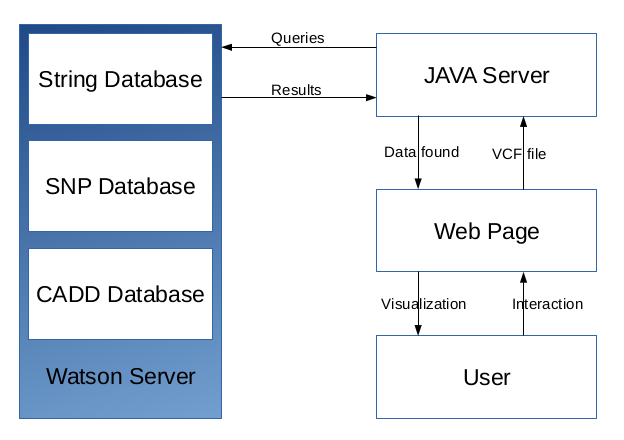
\includegraphics[scale=0.5]{schema1.png}
		\begin{itemize}
			\item Watson server
				\subitem The Watson server owned by the TU Delft hosts the databases string\cite{franceschini2013string}, dbSNP\cite{sherry2001dbsnp} and CADD\cite{kircher2014general} and processes queries given by the JAVA server and returns the results.
			\item Java server
				\subitem The java server makes queries and sends these to Watson. It makes these based on the VCF-file given by the web page. It processes these and determines which data is to be retrieved. The data retrieved is then sent to the web page.
			\item Website
				\subitem The website receives the VCF-file from the user and passes it on to the JAVA server. When it receives data back from the server it visualizes this for the user.
			\item The user 
				\subitem The user can interact with the website and pick a VCF-file to send. The web page outputs a visualization and the user can draw conclusions from this.
		\end{itemize}
	\subsection{Hardware/software mapping}
		This system will only be used by one type of person, namely a doctor. This means that only one interface will have to be developed and used. A user needs to log on to a web page, after which he or she will be shown a page where VCF-files can be uploaded and analyzed. The web page can be accessed from devices connected to the Internet but is targeted at desktops.
	\subsection{Database Connectivity}
		dbSNP\\
		String\\
		CADD\\
		User \& patients database\\\\
		We use an extra database hosted at the webserver to store extra information for the webapplication. 
		The credentials of the users, the doctors, are stored in the database, the passwords are hashed and salted.
		Each user can have multiple patients which are linked through the id of the user.
		Some basic information is stored per user including the uploaded VCF-file.
		For every patient the mutations found in the VCF-file are stored as a single mutation, which is linked to each patient with the patient id.
		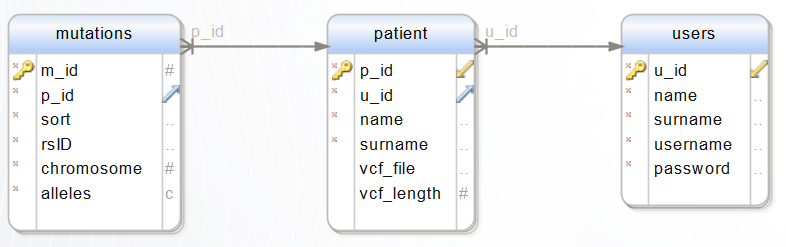
\includegraphics[scale=0.5]{erd.png}
		Old v\\
		The only data our application handles are VCF-files sent by users. We currently have no plans to fill a database with these files for each user. We might give the user the option to export the data of the visualization so that he or she can view this later. We try to keep the data in the JAVA server as low as possible, to support more users.
	\subsection{Concurrency }
		At the moment we have no indication how computationally intense our calculations are, thus we cannot say for sure whether or not we will use multiple threads. Until we know more, our program will run on a single thread.
		
